\documentclass{beamer}

\usetheme{Madrid}

\usepackage[utf8]{inputenc}
\usepackage[T1]{fontenc}
\usepackage{float}
\usepackage{listings}
\usepackage{amsmath}
\usepackage{amssymb}
\usepackage[mathcal]{euscript}

\newcommand{\source}[1]{\caption*{Source: {#1}} }

\title[The BLS Signature Scheme]{The BLS Signature Scheme}
\author[Gabor Tanz]{Gabor Tanz}
\institute[BFH]{Berne University of Applied Sciences}
\date[2019]{2019}

\AtBeginSection[]
{
	\begin{frame}
		\frametitle{Table of Contents}
		\tableofcontents[currentsection]
	\end{frame}
}

\begin{document}

\frame\titlepage

\begin{frame}
	\frametitle{Table of Contents}
	\tableofcontents
\end{frame}

\section{Introduction}
\begin{frame}{Introduction}
	What is BLS?
	\begin{itemize}
		\item Signature method based on bilinear pairing in an EC group
		\item Invented by Boneh, Lynn and Shacham
		\item Uses Weil pairing
		\item Has short signatures
		\item And more (later)
	\end{itemize}
\end{frame}
\section{Prerequisites}
\subsection{Elliptic curves}
\begin{frame}{Elliptic curves}
	Basics
	\begin{itemize}
		\item Set of points satisfying $y^2 = x^3 + ax + b$
		\item Defined over $\mathbb{F} = (F, +, -, 0, *, ^{-1}, 1)$
	\end{itemize}
	\begin{figure}[hbt!]
		\centering
		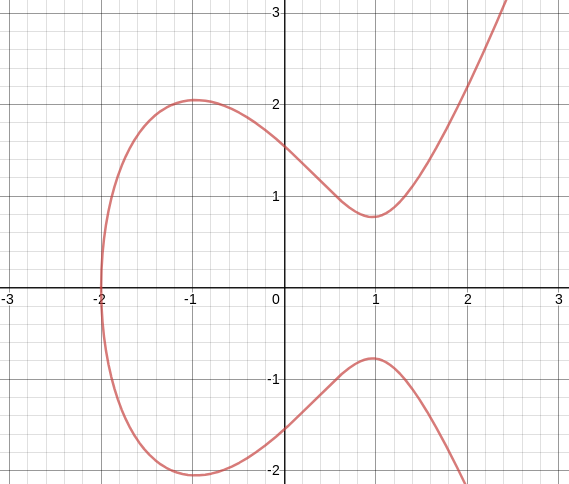
\includegraphics[width=0.5\linewidth]{ec1}
		\caption[]{Example of an elliptic curve: $y^2 = x^3 - 2.8x + 2.4$}
		\label{fig:ec-b2}
	\end{figure}
\end{frame}
\begin{frame}{Elliptic curves}
	Addition of points
	\begin{itemize}
		\item intersection always at 3 points (tangential counts twice)
		\item addition of $P$ and $Q$ is mirror of 3rd intersection
	\end{itemize}
	\begin{figure}[hb!]
		\centering
		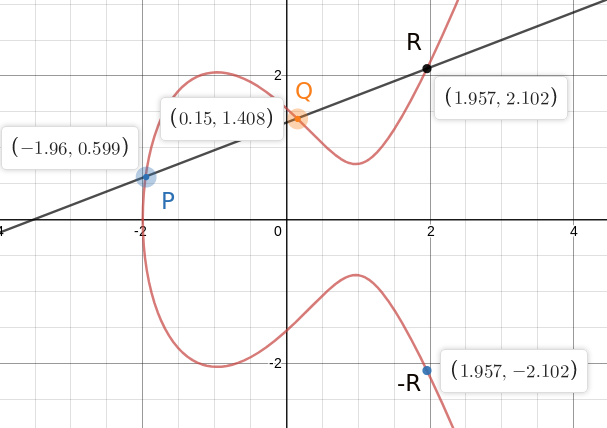
\includegraphics[width=0.5\linewidth]{ec2}
		\caption[]{Example with $P, Q, R$ and $-R$}
	\end{figure}
\end{frame}
\begin{frame}{Elliptic curves}
	EC over finite Fields
	\begin{itemize}
		\item Field given by $(\mathbb{Z}_p,+,-,0,\times,^{-1},1)$ if $p$ with $p$ being prime
		\item Points repeat (wraparound)
	\end{itemize}
	\begin{figure}[hbt!]
		\centering
		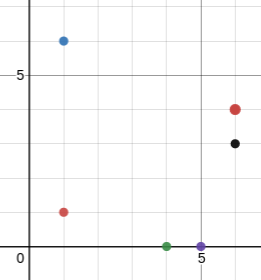
\includegraphics[width=0.4\linewidth]{ec3}
		\caption{$y^2 \equiv x^3 + 2x + 5$ mod $7$}
	\end{figure}
\end{frame}
\subsection{Bilinear maps}
\begin{frame}{Bilinear maps}
	\begin{itemize}
		\item Maps two additive groups $G$ of $ord(p)$ to multiplicative target Group $G_t$ $e: G_1 \times G_2 \rightarrow G_t$
		\item commutativity for additive and multiplicative operations
		\item distributivity for multiplicative operations
		\item $e(u^a,v^b) = e(u^b,v^a)$ as $e(u,v)^{ab} = e(u,v)^{ba}$ or $e(a\times{u},b\times{v}) = e(u,ab\times{v}) = e(ab\times{u},v) = e(u,v)^{ab}$
	\end{itemize}
	\begin{figure}[hbt!]
		\centering
		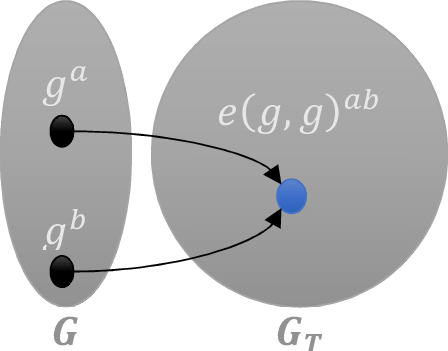
\includegraphics[width=0.25\linewidth]{pairing1}
		\caption{illustration of pairing}
	\end{figure}
\end{frame}
\section{Signature schemes}
\subsection{Key generation}
\begin{frame}{Key generation}
	\begin{itemize}
	\item Generates public and private key
	\item Privatekey should be random
	\item Impossible to derive private from public key
	\item $G(n) := sk \text{ and } pk.$
	\end{itemize}
\end{frame}
\subsection{Signature generation}
\begin{frame}{Signature generation}
	\begin{itemize}
		\item Input: private key and message
		\item Output: signature
		\item Usually signature of Hash(m) is generated
		\item $S(sk, m) := \sigma$
	\end{itemize}
\end{frame}
\subsection{Signature validation}
\begin{frame}{Signature validation}
	\begin{itemize}
		\item Input: message, public key and signature
		\item Output: true or false
		\item $V(pk, m, \sigma) := \text{ true or false}$
	\end{itemize}
\end{frame}
\subsection{Hash functions}
\begin{frame}{Hash functions}
	\begin{itemize}
		\item Input: message of arbitrary size
		\item Output: Value(Hash) of fixed size
		\item Not reversible
		\item Same input will result in same output
	\end{itemize}
\end{frame}
\section{BLS signatures}
\begin{frame}{BLS signatures}
	\begin{itemize}
		\item Hashes directly to the curve
		\item Not every Hash result is valid curve point
		\item Append incrementing value until curve point found
	\end{itemize}
	\begin{figure}[hbt!]
		\centering
		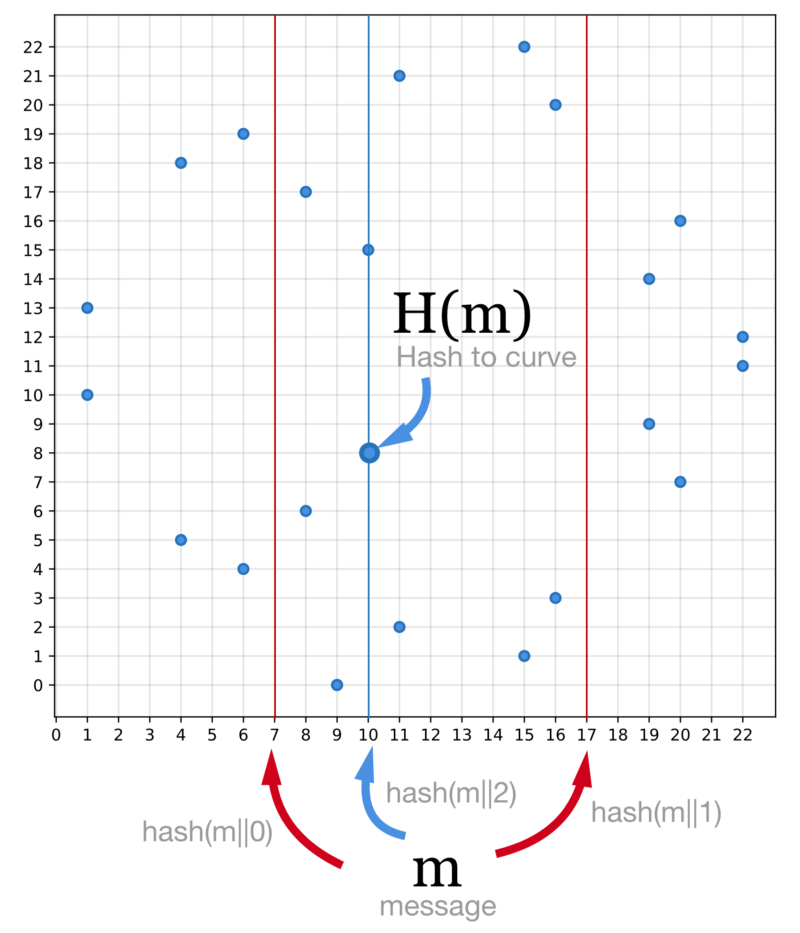
\includegraphics[width=0.35\linewidth]{bls-hash}
		\caption{Hashing on the curve $y^2=x^3+7$ mod 23}
	\end{figure}
\end{frame}
\begin{frame}{BLS signatures}
	Functions:
	\begin{itemize}
		\item KeyGen $G()$: $sk$ -> random, $pk = sk \times{G}$, G := generator Point
		\item SigGen $S(sk, m)$: $\sigma\ := h\times{sk}$ and $h := H(m)$		
	\end{itemize}
	\begin{figure}[hbt!]
		\centering
		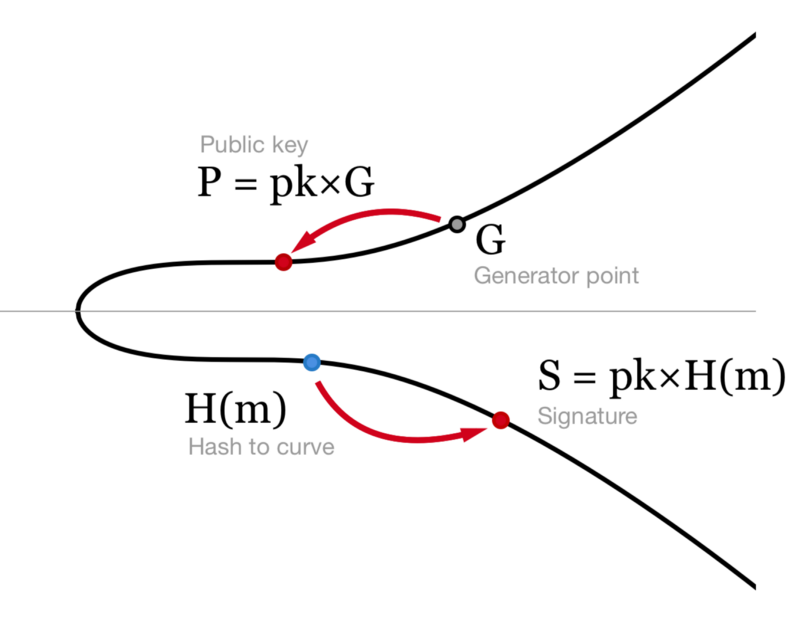
\includegraphics[width=0.4\linewidth]{bls-sign}
		\caption{BLS signature generation, note: P=pk pk=sk S=$\sigma$}
	\end{figure}
\end{frame}
\begin{frame}{BLS signatures}
	Signature Validation
	\begin{itemize}
		\item $V(pk, m, \sigma)$: Check $e(pk,H(m)) = e(G,\sigma)$
		\item works because $e(pk,H(m)) = e(sk\times{G},H(m)) = e(G,sk\times{H(m)}) = e(G, \sigma)$.
	\end{itemize}
	\begin{figure}[hb!]
		\centering
		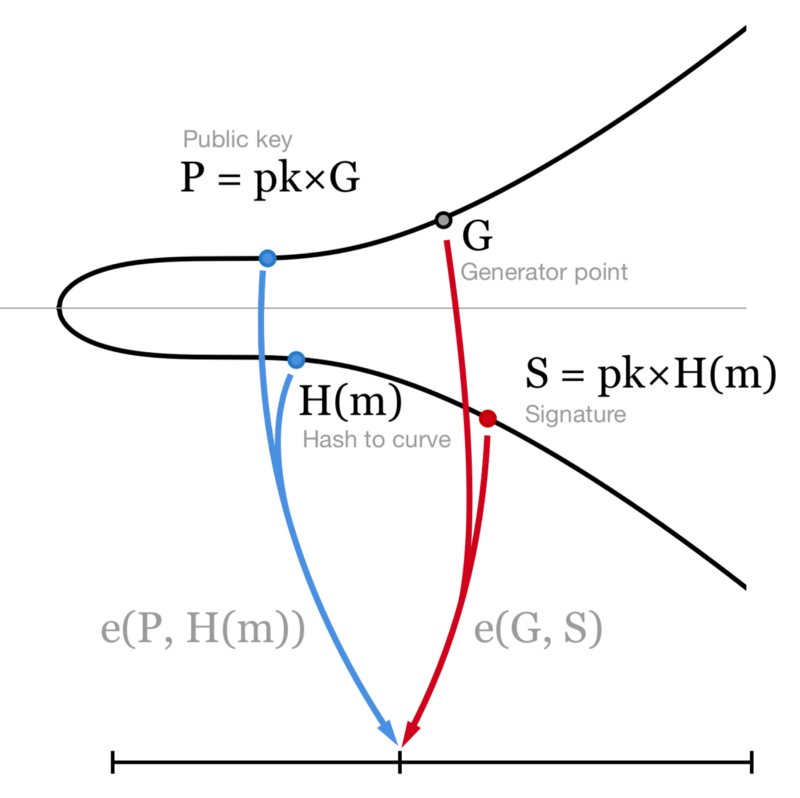
\includegraphics[width=0.37\linewidth]{bls-verify}
		\caption{BLS signature validation, note: P=pk pk=sk S=$\sigma$ \newline
			{\tiny Pictures are from https://medium.com/cryptoadvance/bls-signatures-better-than-schnorr-5a7fe30ea716}}
	\end{figure}
\end{frame}
\subsection{Signature aggregation}
\begin{frame}{Signature aggregation}
	\begin{itemize}
		\item All primitves ($sk, pk, \sigma$) can be aggregated if of same type
		\item Aggregate will be of same type
		\item Aggregates can be aggregated
	\end{itemize}
\end{frame}
\subsection{Threshold signatures}
\begin{frame}{Threshold signatures}
	\begin{itemize}
		\item m-of-n signatures
		\item need only m signature shares to generate signature created from n signature shares
		\item needs setup phase in BLS and normal hashing in addition to curve hashing (once)
		\item blinding to prevent rogue key attacks
		\item generates aggregated $pk$ and membership key $M_i$ for signing
	\end{itemize}
\end{frame}
\begin{frame}{Threshold signatures}
	Example
	\begin{itemize}
		\item Setup \newline
		$a_i = hash(pk_i,{pk_1,pk_2,pk_3})$ \newline
		$pk = a_1\times{pk_1}+a_2\times{pk_2}+a_3\times{pk_3}$ \newline
		$M_i = (a_1 \cdot sk_1) \times{H(pk,i)} + (a_2 \cdot sk_2) \times{H(pk,i)} + (a_3 \cdot sk_3) \times{H(pk,i)}$ \newline
		$e(G,M_i) = e(pk,H(pk,i))$
		\item Sign \newline
		$\sigma_1 = sk_1 \times{H(pk,m)} + M_1$ and $\sigma_2 = sk_2 \times{H(P,m)} + M_2$
		$(\sigma',pk') = (\sigma_1 + \sigma_2, pk_1 + pk_2)$.
		\item Validate \newline
		$e(G,\sigma') = e(pk',H(pk,m)) \cdot e(pk, H(pk,1)+H(pk,2))$
	\end{itemize}
\end{frame}
\section{Usage of BLS for cryptocurrencies}
\begin{frame}{Splitting of private key}
	\begin{itemize}
		\item User can split his private key to $n$ shares
		\item Public address is still public key of original private key
		\item indistinguishable from normal address
		\item even if found out(out of band) that it splitted, no knowledge of \#keyshares
	\end{itemize}
\end{frame}
\begin{frame}{Multiparty signatures}
	\begin{itemize}
		\item Multiple keys can sign a transaction which can be aggregated
		\item Transaction is only valid if at least m-of-n signatures are valid
		\item Demonstrated in earlier example
		\item Doesn't need merkle tree of public keys
		\item Doesn't need several communication rounds
	\end{itemize}
\end{frame}
\begin{frame}{Signature aggregation of transaction blocks}
	\begin{itemize}
		\item Typical transaction has message, pubkey, signature
		\item Block consists of transactions
		\item Block is valid if all transactions have valid signatures
		\item Signatures can be aggregated and just store aggregate signature (size of 1 signature) \newline
		 $\sigma = \sigma_1 + \sigma_2 + ... + \sigma_{1000}$
		 \item Can be validated via \newline
		 $e(G,\sigma) = e(pk_1,H(m_1)) \cdot e(pk_2,H(m_2)) \cdot ... \cdot e(pk_{1000},H(m_{1000}))$
	\end{itemize}
\end{frame}
\section{Conclusion}
\begin{frame}{Conclusion}
	\begin{itemize}
		\item Complicated math with useful properties
		\item Could reduce size of blocks
		\item Better privacy with splitted keyshares
		\item Easier multiparty signatures
	\end{itemize}
\end{frame}

\end{document}
